\documentclass{standalone}

\usepackage{tikz}
\usepackage{pgfplots}

\usetikzlibrary{calc}

\begin{document}
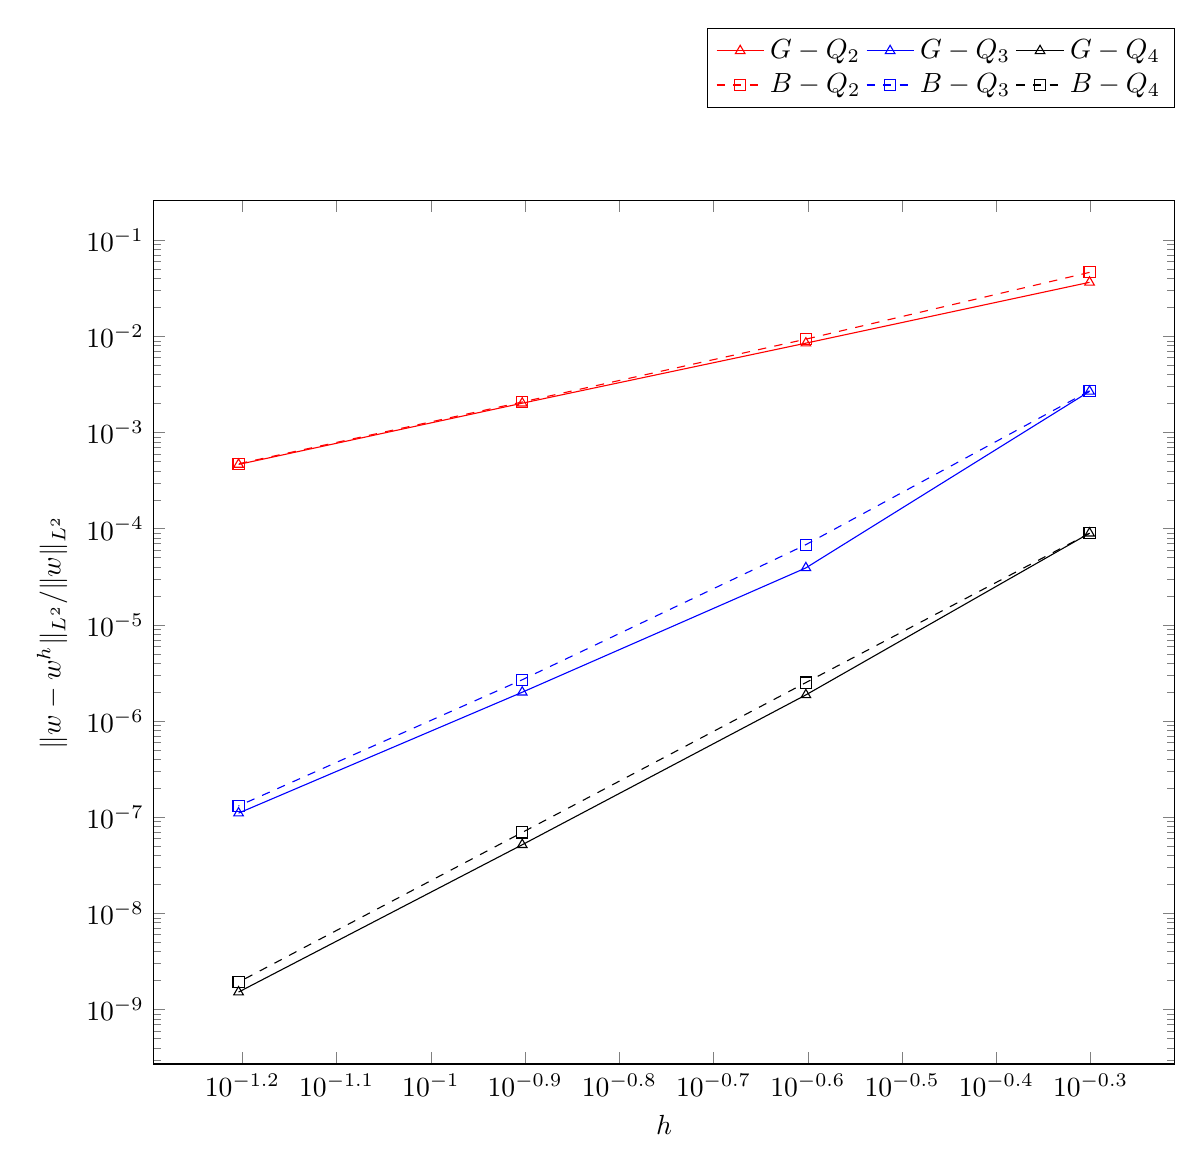
\begin{tikzpicture}
    \begin{loglogaxis}[
        legend columns=3,
    	legend style={at={(1,1.2)}, nodes={scale=1, transform shape}},
        xlabel=$h$,
        ylabel=${\|w-w^{h}\|_{L^2}}/{\|w\|_{L^2}}$ ,
        width=1.2\textwidth
    ]

    \addplot [color=red,mark=triangle] plot coordinates {

        (.5,        0.03653)
        (.25,       0.00850892)
        (.125,      0.00202032)
        (.0625,     0.000466517)
    };

    
    \addplot [color=blue,mark=triangle] plot coordinates {

        (.5,        0.00268351)
        (.25,       3.91737e-05)
        (.125,      1.9954e-06)
        (.0625,     1.10387e-07)
    };

    \addplot [color=black,mark=triangle] plot coordinates {

        (.5,        8.99182e-05)
        (.25,       1.87226e-06)
        (.125,      5.17828e-08)
        (.0625,     1.52153e-09)
    };

    \addplot [color=red,mark=square, every mark/.append style={solid}, dashed] plot coordinates {

        (.5,        0.0463388)
        (.25,       0.00936275)
        (.125,      0.00208014)
        (.0625,     0.000474286)
    };

    
    \addplot [color=blue,mark=square, every mark/.append style={solid}, dashed] plot coordinates {

        (.5,        0.00271825)
        (.25,       6.83176e-05)
        (.125,      2.69025e-06)
        (.0625,     1.31228e-07)
    };

    \addplot [color=black,mark=square, every mark/.append style={solid}, dashed] plot coordinates {

        (.5,        8.97131e-05)
        (.25,       2.51466e-06)
        (.125,      6.95279e-08)
        (.0625,     1.92924e-09)
    };

    \logLogSlopeTriangle{0.25}{0.17}{0.06}{5}{black};
    \logLogSlopeTriangle{0.25}{0.17}{0.28}{4}{blue};
    \logLogSlopeTriangle{0.25}{0.17}{0.68}{2}{red};

    \legend{$G-Q_2$\\$G-Q_3$\\$G-Q_4$\\$B-Q_2$\\$B-Q_3$\\$B-Q_4$\\}
    \end{loglogaxis}
\end{tikzpicture}

\end{document}
